\section{问题一\nobreak：单典型日确定性最优计划模型}
\label{sec:q1}

\subsection{模型建立}

问题一中电价\nobreak、负载与光伏预测在 0:00 全部已知\nobreak，且要求 0:00 与 24:00 储电量相同\nobreak，
故在通用模型 \eqref{eq:obj}--\eqref{eq:c5} 上取 $\hat L_t=L_t^{\text{附1}}$\nobreak、
$\hat{PV}_t=PV_t^{\text{附1}}$\nobreak、$p_t=p_t^{\text{附1}}$\nobreak，并施加端点约束
\begin{equation}
E_1 = E_{145} = 6000\ \text{kWh},
\label{eq:q1end}
\end{equation}
去掉残值项\nobreak。该模型共 577 个变量\nobreak、289 条约束\nobreak，用 HiGHS 求解约 9 ms\nobreak，
\textbf{残差最大值 $1.1\times10^{-13}$ kWh}\nobreak，SOC 全程位于 $[1200,10800]$ 且触及上下限\nobreak，
无同时充放电时段\nobreak，说明解在物理上完全可行且约束均被有效利用\nobreak。

\subsection{求解结果}

\begin{table}[htbp]
\centering
\caption{问题一\nobreak：指定时段的购电量及全天购电量与购电费（表 1 格式\nobreak）}
\label{tab:q1a}
\zihao{-5}
\begin{tabular}{@{}lrlrlr@{}}
\toprule
时间段 & 购电量(kWh) & 时间段 & 购电量(kWh) & 时间段 & 购电量(kWh) \\
\midrule
10:00--10:10 & 0.00 & 12:00--12:10 & 480.41 & 14:00--14:10 & 0.00 \\
16:00--16:10 & 445.43 & 18:00--18:10 & 531.89 & 20:00--20:10 & 0.00 \\
\multicolumn{2}{l}{\textbf{全天购电量}} & \multicolumn{4}{l}{\textbf{59\,482.67 kWh}} \\
\multicolumn{2}{l}{\textbf{全天购电费}} & \multicolumn{4}{l}{\textbf{35\,126.95 元}} \\
\bottomrule
\end{tabular}
\end{table}

\begin{table}[htbp]
\centering
\caption{问题一\nobreak：储能设备分时段充放电量与 0:00\nobreak、24:00 储电量（表 2 格式\nobreak）}
\label{tab:q1b}
\zihao{-5}
\begin{tabular}{@{}lrrlrr@{}}
\toprule
时间段 & 充电量(kWh) & 放电量(kWh) & 时间段 & 充电量(kWh) & 放电量(kWh) \\
\midrule
0:00--4:00 & 4500.00 & 0.00 & 4:00--8:00 & 833.33 & 6365.84 \\
8:00--12:00 & 4787.96 & 1703.00 & 12:00--16:00 & 5286.04 & 91.10 \\
16:00--20:00 & 0.00 & 5780.13 & 20:00--24:00 & 5333.33 & 2859.87 \\
\midrule
0:00 储电量 & \multicolumn{2}{r}{6000.00 kWh} & 24:00 储电量 & \multicolumn{2}{r}{6000.00 kWh} \\
\bottomrule
\end{tabular}
\end{table}

\begin{figure}[htbp]
\centering
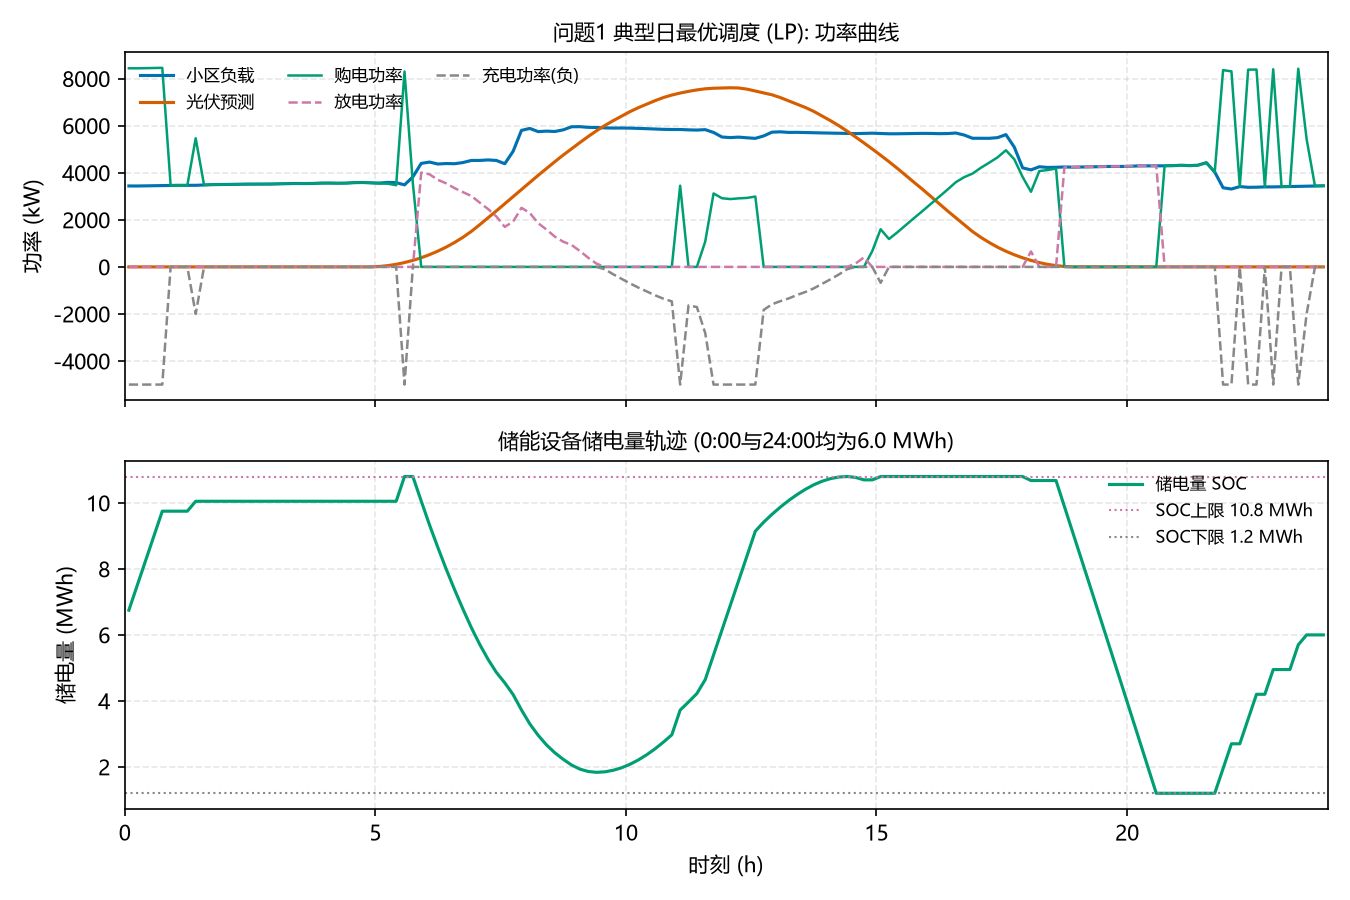
\includegraphics[width=0.86\textwidth]{figures/fig_q1_schedule.png}
\caption{问题一最优调度\nobreak：功率曲线（上\nobreak）与储电量轨迹（下\nobreak）}
\label{fig:q1}
\end{figure}

\subsection{结果分析}

最优策略呈现清晰的“低充高放\nobreak”结构（\cref{fig:q1}\nobreak、\cref{tab:q1a}\nobreak、\cref{tab:q1b}\nobreak）\nobreak：

\begin{enumerate}[label=(\arabic*), leftmargin=2.2em, itemsep=1pt]
\item \textbf{夜间低价充电（0:00--4:00\nobreak，电价均值 0.432 元/kWh\nobreak）}\nobreak：充电 4500 kWh 将储电量由 6000 抬升至 10\,050 kWh\nobreak；
\item \textbf{早高峰放电（4:00--8:00\nobreak，电价均值 0.671 元/kWh\nobreak）}\nobreak：放电 6365.84 kWh 覆盖负载高峰\nobreak，
其边际成本 $0.432/0.81=0.533$ 元/kWh 低于直接购电\nobreak；
\item \textbf{午间弃光充电（8:00--16:00\nobreak）}\nobreak：光伏富余功率为免费电源\nobreak，共充电 10\,074 kWh\nobreak；
\item \textbf{傍晚尖峰放电（16:00--20:00\nobreak，电价均值 1.134 元/kWh\nobreak）}\nobreak：放电 5780.13 kWh 是全天收益最高的动作\nobreak；
\item \textbf{夜间回充并精准归位}\nobreak：20:00--24:00 充电 5333.33 kWh\nobreak，使 24:00 储电量恰好回到 6000 kWh\nobreak，
满足端点约束的同时用尽低价时段\nobreak。
\end{enumerate}

\subsection{方法对照\nobreak：LP 与启发式\nobreak、与无储能基线}

\begin{table}[htbp]
\centering
\caption{问题一三种方法的对照（典型日购电费\nobreak）}
\label{tab:q1cmp}
\zihao{-5}
\begin{tabular}{@{}lccc@{}}
\toprule
方法 & 购电费(元) & 相对 LP & 说明 \\
\midrule
\textbf{线性规划（采用\nobreak）} & \textbf{35\,126.95} & --- & 577 变量精确最优\nobreak，9 ms \\
贪心配对启发式 & 42\,187.93 & +7\,060.98 (+20.1\%) & 忽略充放电时序约束的松弛解 \\
无储能基线 & 48\,052.05 & +12\,925.10 (+36.8\%) & 缺额全部按当时电价购买 \\
\bottomrule
\end{tabular}
\end{table}

\cref{tab:q1cmp} 表明\nobreak：储能使典型日购电费下降 \textbf{26.9\%}（12\,925 元\nobreak）\nobreak；
而启发式即便在“忽略时序约束\nobreak”的宽松条件下仍比 LP 贵 7061 元\nobreak，
印证了第 2 节“本问题应当用 LP 精确求解\nobreak”的判断\nobreak。
